\section{Test sul sistema linearizzato}

    Per testare il sistema di controllo sul sistema linearizzato abbiamo usato simulink, 
    ottenendo il seguente diagramma a blocchi.\\\\
    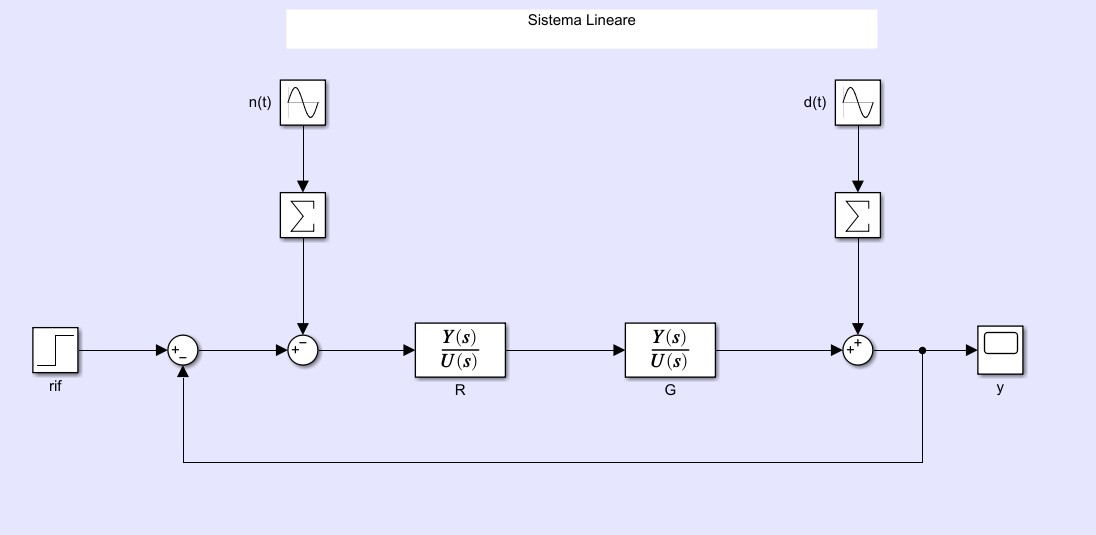
\includegraphics[scale=0.5]{immagini/diaglin.jpg}\\\\
    In particolare ci viene richiesto di testare il sistema con:
    \begin{align*}
        &w(t)=8  \cdot 10^{-5 }\cdot 1(t)\\
        &u(t)=\sum_{k=1}^4 3 \cdot 10^{-5} \cdot \sin(0.02kt)\\
        &n(t)=\sum_{k=1}^4 2 \cdot 10^{-4} \cdot \sin(5 \cdot 10^{4} kt)
    \end{align*}
    Ottenendo come risposta \\
    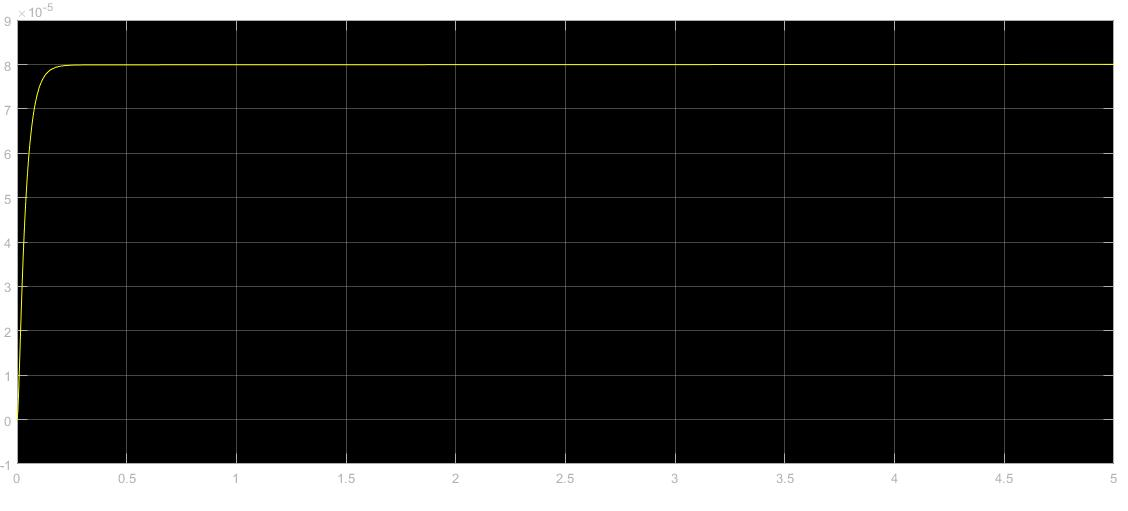
\includegraphics[scale=0.4]{immagini/risplin.jpg}